\section{Matrix Transformations}\label{sec:geom_3}

\asyouread{
\item What do mathematicians do?
\item T/F: Multiplying a vector by a matrix always changes its length and direction.
%\item	T/F: Transforming the Cartesian plane through matrix multiplication makes curved lines straight.
%\item T/F: To understand how the Cartesian plane is affected by multiplication by a matrix, it helps to know how the unit square is affected.
\item		To understand how the Cartesian plane is affected by multiplication by a matrix, it helps to study how what is affected?
\item		Transforming the Cartesian plane through matrix multiplication transforms straight lines into what kind of lines?
\item T/F: If one draws a picture of a sheep on the Cartesian plane, then transformed the plane using the matrix 
\[
\bmx{cc} -1&0\\0&1\emx,
\]
one could say that the sheep was ``sheared.''
}

We already looked at the basics of graphing vectors, and the arithmetic of multiplying matrices. In this section and the next, we will return to the geometric interpretation of vectors given in Chapter \ref{chapter:vectors}. Our goal in doing so is to obtain a visual understanding of the definition of matrix multiplication given in Section \ref{sec:matrix_multiplication}. Although the algebraic definition of matrix multiplication appears strange at first, we'll see that our definition of matrix multiplication allows us to use matrices to define \sword{functions} that transform one vector into another, just as the functions you're familiar with from high school or Calculus transform one number into another. We can then visualize matrices and matrix multiplication in terms of their effect on vectors.

Given an $m\times n$ matrix $A$ we can define a function $T$ that takes an $n\times 1$ column vector $\vec x\in \mathbb{R}^n$ as input, and produces an $m\times 1$ column vector $\vec y\in \mathbb{R}^m$ as output, according to the relationship
\[
\vec y = T(\vec x) = A\vec x.
\]
Such a function is known as a \sword{matrix transformation}\index{matrix transformation}\index{transformation ! matrix}; it is an example of a more general class of functions between vector spaces known as \sword{linear transformations}.

The graphical representation of vectors allows us to visualize matrix transformations (at least, in lower dimensions). This visualization plays a key role in applications such as computer graphics. We'll also see that the desire to define functions via matrix multiplication provides some justification for defining matrix multiplication the way we do.

\subsection*{Matrix - Vector Multiplication}
To simplify the discussion, and to make it easier for us to picture what's going on, we'll restrict ourselves (for now) to vectors in $\mathbb{R}^2$. We want to visualize the result of multiplying a vector by a matrix. In order to multiply a 2D vector by a matrix and get a 2D vector back, our matrix must be a square, $2\times 2$ matrix.

\mnote{.5}{We can multiply a $3\times 2$ matrix by a 2D vector and get a 3D vector back, and this gives very interesting results. See section \ref{sec:lin_trans}.}

We'll start with an example. Given a matrix \tta\ and several vectors, we'll graph the vectors before and after they've been multiplied by \tta\ and see what we learn.

\medskip

\example{ex_mv_1}{Multiplying a vector by a matrix}{Let \tta\ be a matrix, and \vx, \vy, and \vz\ be vectors as given below.
\[
\tta = \bmx{cc} 1&4\\2&3\emx,  \quad \vx = \bmx{c} 1\\1\emx, \quad \vy = \bmx{c}-1\\1\emx, \quad \vz = \bmx{c} 3\\-1\emx
\]
Graph \vx, \vy\ and \vz, as well as \tta\vx, \tta\vy\ and \tta\vz.}
{\begin{myfigure}%[h!]
\begin{center}
\begin{tikzpicture}[x={(.6cm,0)},y={(0,.6cm)}, >=latex]

\drawxlines{-2.5}{6.5}{-2,...,6};
\drawylines{-1.5}{5.5}{-1,...,5};
\draw [->] (0,0)--(1,1) node [right ] {\vx};
\draw [->] (0,0)--(-1,1) node [above] {\vy};
\draw [->] (0,0)--(3,-1) node [below right] {\vz};
\draw [->] (0,0)--(5,5) node [above right] {\tta\vx};
\draw [->] (0,0)--(3,1) node [right] {\tta\vy};
\draw [->] (0,0)--(-1,3) node [above] {\tta\vz};

\end{tikzpicture}
\end{center}
\mycaption{Multiplying vectors by a matrix in Example \ref{ex_mv_1}.}
\label{fig:mv_1}
\end{myfigure}%

It is straightforward to compute: 
\[
\tta\vx = \bmx{c} 5\\5\emx,\quad \tta\vy = \bmx{c} 3\\1\emx, \quad \text{ and } \quad \tta\vz = \bmx{c} -1\\3\emx.
\]
The vectors are sketched in Figure \ref{fig:mv_1}
}

\medskip

There are several things to notice. When each vector is multiplied by \tta, the result is a vector with a different length (in this example, always longer), and in two of the cases (for \vy\ and \vz), the resulting vector points in a different direction. 

This isn't surprising. In the previous section we learned about matrix multiplication, which is a strange and seemingly unpredictable operation. Would you expect to see some sort of immediately recognizable pattern appear from multiplying a matrix and a vector? (This is a rhetorical question; the expected answer is ``No.'') In fact, the surprising thing from the example is that \vx\ and \tta\vx\ point in the same direction! Why does the direction of \vx\ not change after multiplication by \tta? (We'll answer this in Section \ref{sec:eigen} when we learn about something called ``eigenvectors.'')

%One may recall that \tta\ and \vx\ previously appeared in Section \ref{sec:eigen}, where \vx\ is an eigenvector of \tta\ with an \el\ of 5. Therefore this example lets us visualize the significance of \ev s: ``normally,'' when a vector is multiplied by a matrix, its length and direction changes. However, when the vector is an \ev, its direction does not change, only its length\footnote{If the \el\ is 1, then of course, nothing changes. The careful reader will also note that if the $\el <0$, then the resulting vector will point in the opposite direction, meaning the direction \textit{did} change. However, in this case, \vx\ and \tta\vx\ lie on the same line which is still significant}.

Different matrices act on vectors in different ways. (That's one reason we call them ``different.'') Some always increase the length of a vector through  multiplication, others always decrease the length, others increase the length of some vectors and decrease the length of others, and others still don't change the length at all. A similar statement can be made about how matrices affect the direction of vectors through multiplication: some change every vector's direction, some change ``most'' vector's direction but leave some the same, and others still don't change the direction of any vector.

How do we set about studying how matrix multiplication affects vectors? We could just create lots of different matrices and lots of different vectors, multiply, then graph, but this would be a lot of work with very little useful result. It would be too hard to find a pattern of behaviour in this. (Remember, that's what mathematicians do. We look for patterns.)

Instead, we'll begin by using a technique we've employed often in the past. We have a ``new'' operation; let's explore how it behaves with ``old'' operations. Specifically, we know how to sketch vector addition. What happens when we throw matrix multiplication into the mix? Let's try an example.

\medskip

\example{ex_mv_2}{Combining addition and matrix multiplication}{Let \tta\ be a matrix and \vx\ and \vy\ be vectors as given below. 
\[
\tta = \bmx{cc} 1 & 1\\1&2\emx, \quad \vx = \bmx{c} 2\\1\emx, \quad \vy = \bmx{c} -1\\1\emx
\]
Sketch $\vx+\vy$, \tta\vx, \tta\vy, and $\tta(\vx+\vy)$. }
{It is pretty straightforward to compute: 
\[
\vx+\vy = \bmx{c} 1\\2\emx;\quad \tta\vx = \bmx{c}3\\4\emx; \quad \tta\vy = \bmx{c} 0\\1\emx,\quad \tta(\vx+\vy) = \bmx{c} 3\\5\emx.
\]

In Figure \ref{fig:mv_2}, we have graphed the above vectors and have included dashed gray vectors to highlight the additive nature of $\vx+\vy$ and $\tta(\vx+\vy)$. Does anything strike you as interesting?

\begin{myfigure}%[h!]
\begin{center}
\begin{tikzpicture}[x={(1cm,0)},y={(0,1cm)}, >=latex]
\drawxlines{-1}{4}{0,...,3};
\drawylines{-1}{5}{0,...,4};
\draw [->] (0,0)--(2,1) node [right] {\vx};
\draw [->] (0,0)--(-1,1) node [left ] {\vy};
\draw [->,gray,dashed] (2,1) -- (1,2);
\draw [->] (0,0)--(1,2) node [above] {$\vx+\vy$};
\draw [->] (0,0)--(3,4) node [above right] {\tta\vx};
\draw [->] (0,0)--(0,1) node [above left] {\tta\vy};
\draw [->,gray,dashed] (3,4) -- (3,5);
\draw [->] (0,0)--(3,5) node [above] {$\tta(\vx+\vy)$};
\end{tikzpicture}
\end{center}
\mycaption{Vector addition and matrix multiplication in Example \ref{ex_mv_2}.}
\label{fig:mv_2}
\end{myfigure}%

Let's not focus on things which don't matter right now: let's not focus on how long certain vectors became, nor necessarily how their direction changed. Rather, think about how matrix multiplication interacted with the vector addition.

In some sense, we started with three vectors, \vx, \vy, and $\vx+\vy$. This last vector is special; it is the sum of the previous two. Now, multiply all three by \tta. What happens? We get three new vectors, but the significant thing is this: the last vector is still the sum of the previous two! (We emphasize this by drawing dotted vectors to represent part of the Parallelogram Law.)

Of course, we knew this already: we already knew that $\tta\vx + \tta\vy = \tta(\vx+\vy)$, for this is just the Distributive Property of matrix multiplication given in Theorem \ref{thm:matrix_multiplication}. However, now we get to see this graphically.}

\medskip

Let's do one more example.

\medskip


\example{ex_mv_23}{Sketching the effect of matrix multiplicaiton}{Let \tta, \vx, \vy, and \vz\ be as given below.
\[
\tta = \bmx{cc} 1&-1\\1&-1\emx,  \quad \vx = \bmx{c} 1\\1\emx, \quad \vy = \bmx{c}-1\\1\emx, \quad \vz = \bmx{c} 4\\1\emx
\]
Graph \vx, \vy\ and \vz, as well as \tta\vx, \tta\vy\ and \tta\vz.}
{\begin{myfigure}%[h!]
\begin{center}
\begin{tikzpicture}[x={(.6cm,0)},y={(0,.6cm)}, >=latex]

\drawxlines{-2.5}{3.5}{-2,...,3};
\drawylines{-2.5}{3.5}{-2,...,3};
\draw [->] (0,0)--(1,1) node [right ] {\vx};
\draw [->] (0,0)--(-1,1) node [above] {\vy};
\draw [->] (0,0)--(4,1) node [above] {\vz};
\draw (0,0) node [below right] {\tta\vx};
\draw [->] (0,0)--(-2,-2) node [below left] {\tta\vy};
\draw [->] (0,0)--(3,3) node [above] {\tta\vz};

\end{tikzpicture}
\end{center}
\mycaption{Multiplying vectors by a matrix in Example \ref{ex_mv_23}.}
\label{fig:mv_23}
\end{myfigure}%

It is straightforward to compute: 
\[
\tta\vx = \bmx{c} 0\\0\emx,\quad \tta\vy = \bmx{c} -2\\-2\emx, \quad \text{ and } \quad \tta\vz = \bmx{c} 3\\3\emx.
\]

The vectors are sketched in Figure \ref{fig:mv_23}.

These results are interesting. While we won't explore them in great detail here, notice how \vx\ got sent to the zero vector. Notice also that \tta\vx, \tta\vy\ and \tta\vz\ are all in a line (as well as \vx!). Why is that? Are \vx, \vy\ and \vz\ just special vectors, or would any other vector get sent to the same line when multiplied by \tta? (Don't just sit there, try it out!)
}

\medskip

\subsection*{Transformations of the Cartesian Plane}

We studied in Chapter \ref{chapter:vectors} how to visualize vectors and how the matrix arithmetic operations of addition and scalar multiplication can be graphically represented for vectors. In the discussion above, we limited our visual understanding of matrix  multiplication to graphing a vector, multiplying it by a matrix, then graphing the resulting vector. In rest of this section we'll explore these multiplication ideas in greater depth. Instead of multiplying individual vectors by a matrix \tta, we'll study what happens when we multiply \textit{every} vector in the Cartesian plans by \tta. (No, we won't do them one by one.)

Because of the Distributive Property, as illustrated in Example \ref{ex_mv_2}, we know that the Cartesian plane will be \textit{transformed} in a very nice, predictable way. Straight lines will be transformed into other straight lines (and they won't become curvy, or jagged, or broken). Curved lines will be transformed into other curved lines (perhaps the curve will become ``straight,'' but it won't become jagged or broken).

Example \ref{ex_mv_2} has very significant implications. We usually think of the Cartesian plane as a set of points; we can adjust this thought just slightly and think of it as a set of vectors that point to each of these points. What happens to the Cartesian plane if we multiply \textit{every vector} in the plane by the same matrix \tta? 

Checking every single vector in the plane isn't practical, so we have to look for other ways to visualize the effects of matrix multiplication. One way of studying how the whole Cartesian plane is affected by multiplication by a matrix \tta\ is to study how the \textit{unit square} is affected. The unit square is the square with corners at the points $(0,0)$, $(1,0)$, $(1,1)$, and $(0,1)$. Each corner can be represented by the vector that points to it; multiply each of these vectors by \tta\ and we can get an idea of how \tta\ affects the whole Cartesian plane. 

Let's try an example.

\medskip

\example{ex_mv_3}{Visualizing a matrix transformation using vectors}{Plot the vectors of the unit square before and after they have been multiplied by \tta, where 
\[
\tta = \bmx{cc} 1&4\\2&3\emx.
\] }
{The four corners of the unit square can be represented by the vectors 
\[
\bmx{c}0\\0\emx, \quad \bmx{c}1\\0\emx,\quad \bmx{c}1\\1\emx,\quad \bmx{c}0\\1\emx.
\]
Multiplying each by \tta\ gives the vectors 
\[
\bmx{c}0\\0\emx,\quad \bmx{c} 1\\2\emx,\quad\bmx{c}5\\5\emx,\quad \bmx{c}4\\3\emx,
\]
respectively. 

%\drawexampleline{ex_mv_3}

(Hint: one way of using your calculator to do this for you quickly is to make a $2\times 4$ matrix whose columns are each of these vectors. In this case, create a matrix 
\[
\ttb = \bmx{cccc}0&1&1&0\\0&0&1&1\emx.
\]
Then multiply \ttb\ by \tta\ and read off the transformed vectors from the respective columns: 
\[
\tta\ttb = \bmx{cccc}0&1&5&4\\0&2&5&3\emx.
\]
This saves time, especially if you do a similar procedure for multiple matrices \tta. Of course, we can save more time by skipping the first column; since it is the column of zeros, it will stay the column of zeros after multiplication by \tta.)

The unit square and its transformation are graphed in Figure \ref{fig:mv_3}, where the shaped vertices correspond to each other across the two graphs. Note how the square got turned into some sort of quadrilateral (it's actually a parallelogram). A really interesting thing is how the triangular and square vertices seem to have changed places -- it is as though the square, in addition to being stretched out of shape, was flipped. 
%
%
%
\begin{myfigure}
\begin{center}
\begin{tikzpicture}[x={(.75cm,0)},y={(0,.75cm)}, >=latex]

\begin{scope}
	\drawxlines{-1}{5}{0,...,4};
	\drawylines{-1}{5}{0,...,4};
	\node[below] at (1,-0.1) {1};
	\node[left] at (0,1) {1};
	\unitsquare[very thick];
\end{scope}
\begin{scope}[shift={(7,0)}]
	\drawxlines{-1}{5}{0,...,4};
	\drawylines{-1}{5}{0,...,4};
	\node[below] at (1,-0.1) {1};
	\node[left] at (0,1) {1};
	\unitsquare[cm={1,2,4,3,(0,0)},very thick];
\end{scope}

\end{tikzpicture}
\end{center}
\mycaption{Transforming the unit square by matrix multiplication in Example \ref{ex_mv_3}.}
\label{fig:mv_3}
\end{myfigure}

\begin{myfigure}
\begin{center}
\begin{tikzpicture}[x={(.75cm,0)},y={(0,.75cm)}, >=latex]

\begin{scope}
	\drawxlines{-1}{5}{0,...,4};
	\drawylines{-1}{5}{0,...,4};
	\node[below] at (1,-0.1) {1};
	\node[left] at (0,1) {1};
	\unitsquare[very thick];
	\filldraw [black!70] (.5,0) circle (2pt);
	\filldraw [black!40] (1,.25) circle (2pt);
	\filldraw [black!20] (1,.75) circle (2pt);
\end{scope}

\begin{scope}[shift={(7,0)}]
	\drawxlines{-1}{5}{0,...,4};
	\drawylines{-1}{5}{0,...,4};
	\node[below] at (1,-0.1) {1};
	\node[left] at (0,1) {1};
	\unitsquare[very thick,cm={1,2,4,3,(0,0)}];
	\filldraw [black!70] (.5,1) circle (2pt);
	\filldraw [black!40] (2,2.75) circle (2pt);
	\filldraw [black!20] (4,4.25) circle (2pt);
\end{scope}

\end{tikzpicture}
\end{center}
\mycaption{Emphasizing straight lines going to straight lines in Example \ref{ex_mv_3}.}
\label{fig:mv_3b}
\end{myfigure}

To stress how ``straight lines get transformed to straight lines,'' consider Figure \ref{fig:mv_3b}. Here, the unit square has some additional points drawn on it which correspond to the shaded dots on the transformed parallelogram. Note how relative distances are also preserved; the dot halfway between the black and square dots is transformed to a position along the line, halfway between the black and square dots.
}

\medskip

Much more can be said about this example. Before we delve into this, though, let's try one more example.

\medskip

\example{ex_mv_4}{Visualizing a matrix transformation using a region}{Plot the transformed unit square after it has been transformed by \tta, where 
\[
\tta = \bmx{cc}0&-1\\1&0\emx.
\]
}
{We'll put the vectors that correspond to each corner in a matrix \ttb\ as before and then multiply it on the left by \tta. Doing so gives:
\begin{align*}
\tta\ttb &= \bmx{cc}0&-1\\1&0\emx \bmx{cccc}0&1&1&0\\0&0&1&1\emx\\
				& = \bmx{cccc}0 & 0&-1&-1\\0&1&1&0\emx
\end{align*}

In Figure \ref{fig:mv_4} the unit square is again drawn along with its transformation by \tta.

\begin{myfigure}
\begin{center}
\begin{tikzpicture}[>=latex]

\begin{scope}
	\drawxlines{-1.5}{1.5}{-1,1};
	\drawylines{-1}{1.5}{1};
	\node[below] at (1,-0.1) {1};
	\node[left] at (0,1) {1};	
	\unitsquare[very thick];
\end{scope}

\begin{scope}[shift={(4,0)}]
	\drawxlines{-1.5}{1.5}{-1,1};
	\drawylines{-1}{1.5}{1};
	\node[below] at (1,-0.1) {1};
	\unitsquare[very thick,cm={0,1,-1,0,(0,0)}];
\end{scope}
\end{tikzpicture}
\end{center}
\mycaption{Transforming the unit square by matrix multiplication in Example \ref{ex_mv_4}.}
\label{fig:mv_4}
\end{myfigure}

Make note of how the square moved. It did not simply ``slide'' to the left; (mathematically, that is called a \sword{translation}) nor did it ``flip'' across the $y$ axis. Rather, it was \sword{rotated} counterclockwise about the origin $90^\circ$. In a rotation, the shape of an object does not change; in our example, the square remained a square of the same size.
}

\medskip

We have broached the topic of how the Cartesian plane can be transformed via multiplication by a $2\times 2$ matrix \tta. We have seen a few examples so far, and our intuition as to how the plane is changed has been informed only by seeing how the unit square changes. Let's explore this further by investigating two questions:
	\begin{enumerate}
	\item		Suppose we want to transform the Cartesian plane in a known way (for instance, we may want to rotate the plane counterclockwise $180^\circ$). How do we find the matrix (if one even exists) which performs this transformation? 
	\item		How does knowing how the unit square is transformed really help in understanding how the entire plane is transformed?
	\end{enumerate}

These questions are closely related, and as we answer one, we will help answer the other.

To get started with the first question, look back at Examples \ref{ex_mv_3} and \ref{ex_mv_4} and consider again how the unit square was transformed. In particular, is there any correlation between where the vertices ended up and the matrix \tta?

If you are just reading on, and haven't actually gone back and looked at the examples, go back now and try to make some sort of connection. Otherwise -- you may have noted some of the following things:
\begin{enumerate}
\item		The zero vector (\zero, the ``black'' corner) never moved. That makes sense, though; $\tta\zero = \zero$. 
\item		The ``square'' corner, i.e., the corner corresponding to the vector $\bmx{c}1\\0\emx$, is always transformed to the vector in the first column of \tta!
\item		Likewise, the ``triangular'' corner, i.e., the corner corresponding to the vector $\bmx{c}0\\1\emx$, is always transformed to the vector in the second column of \tta! (This is less of a surprise, given the result of the previous point.)
\item		The ``white dot'' corner is always transformed to the \textit{sum} of the two column vectors of \tta. (This observation is a bit more obscure than the first three.  It follows from the fact that this corner of the unit square is the ``sum'' of the other two nonzero corners.)
\end{enumerate}

Let's now take the time to understand these four points. The first point should be clear; \zero\ will always be transformed to \zero\ via matrix multiplication. (Hence the hint in the middle of Example \ref{ex_mv_3}, where we are told that we can ignore entering in the column of zeros in the matrix \ttb.)

We can understand the second and third points simultaneously. Let 
\[
\tta = \bmx{cc}a&b\\c&d\emx, \quad \veone = \bmx{c}1\\0\emx \quad \text{ and } \quad \vetwo = \bmx{c}0\\1\emx.
\]
What are \tta\veone\ and \tta\vetwo?

\begin{align*}
\tta\veone &= \bmx{cc}a&b\\c&d\emx\bmx{c}1\\0\emx \\
					&= \bmx{c}a\\c\emx
\end{align*}

\begin{align*}
\tta\vetwo &= \bmx{cc}a&b\\c&d\emx\bmx{c}0\\1\emx \\
					&= \bmx{c}b\\d\emx
\end{align*}

So by mere mechanics of matrix multiplication, the square corner \veone\ is transformed to the first column of \tta, and the triangular corner \vetwo\ is transformed to the second column of \tta. A similar argument demonstrates why the white dot corner is transformed to the sum of the columns of \tta. (Another way of looking at all of this is to consider what $\tta\cdot\tti$ is: of course, it is just \tta. What are the columns of \tti? Just \veone\ and \vetwo.)

Revisit now the question ``How do we find the matrix that performs a given transformation on the Cartesian plane?'' The answer follows from what we just did. Think about the given transformation and how it would transform the corners of the unit square. Make the first column of \tta\ the vector where \veone\ goes, and make the second column of \tta\ the vector where \vetwo\ goes.

Let's practice this in the context of an example.

\medskip

\example{ex_transf_1}{Determining a matrix transformation}{Find the matrix \tta\ that flips the Cartesian plane about the $x$ axis and then stretches the plane horizontally by a factor of two.}
{We first consider $\veone = \bmx{c}1\\0\emx$. Where does this corner go to under the given transformation? Flipping the plane across the $x$ axis does not change \veone\ at all; stretching the plane sends \veone\ to $\bmx{c}2\\0\emx$. Therefore, the first column of \tta\ is $\bmx{c}2\\0\emx$.

Now consider $\vetwo = \bmx{c}0\\1\emx$. Flipping the plane about the $x$ axis sends \vetwo\ to the vector $\bmx{c}0\\-1\emx$; subsequently stretching the plane horizontally does not affect this vector. Therefore the second column of \tta\ is $\bmx{c}0\\-1\emx$. 

Putting this together gives 
\[
\tta = \bmx{cc}2&0\\0&-1\emx.
\]
To help visualize this, consider Figure \ref{fig:transf_1} where a shape is transformed under this matrix. Notice how it is turned upside down and is stretched horizontally by a factor of two. (The gridlines are given as a visual aid.)

\begin{myfigure}
\begin{center}
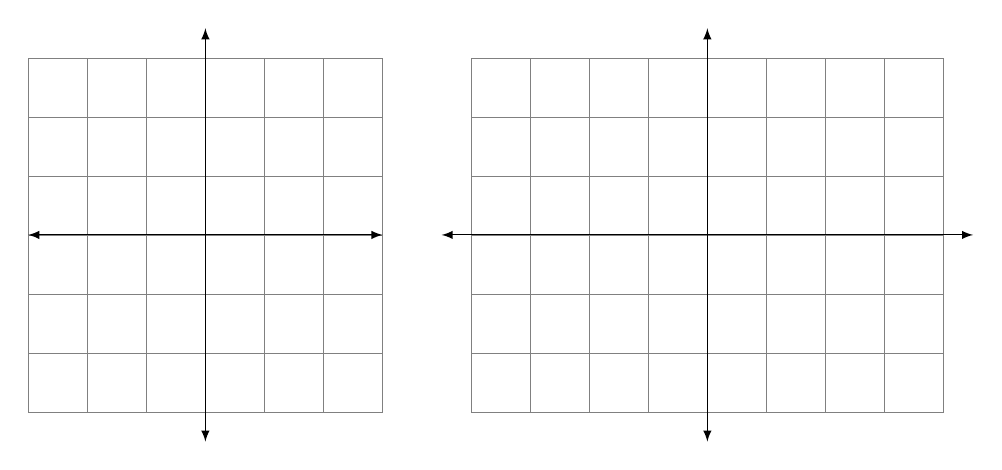
\begin{tikzpicture}[x={(.75cm,0)},y={(0,.75cm)},>=latex]

\begin{scope}
	\draw [ultra thin,gray,step=.75cm] (-3,-3) grid (3,3);
	\draw [<->] (-3,0) -- (3,0);
	\draw [<->] (0,-3.5) -- (0,3.5);
	\vmispider[very thick];
\end{scope}

\begin{scope}[shift={(8.5,0)}]
	\draw [ultra thin,gray,step=.75cm] (-4,-3) grid (4,3);
	\draw [<->] (-4.5,0) -- (4.5,0);
	\draw [<->] (0,-3.5) -- (0,3.5);
	\vmispider[very thick,cm={2,0,0,-1,(0,0)}];
\end{scope}

\end{tikzpicture}
\end{center}
\mycaption{Transforming the Cartesian plane in Example \ref{ex_transf_1}}
\label{fig:transf_1}
\end{myfigure}
\vskip -2\baselineskip}

\medskip

A while ago we asked two questions. The first was ``How do we find the matrix that performs a given transformation?'' We have just answered that question (although we will do more to explore it in the future). The second question was ``How does knowing how the unit square is transformed really help us understand how the entire plane is transformed?'' 

Consider Figure \ref{fig:trans} where the unit square (with vertices marked with shapes as before) is shown transformed under an unknown matrix. How does this help us understand how the whole Cartesian plane is transformed? For instance, how can we use this picture to figure out how the point $(2,3)$ will be transformed?

\begin{myfigure}
\begin{center}
\begin{tikzpicture}[>=latex]
	\drawxlines{-2}{2}{-1,1};
	\drawylines{-1}{3.5}{1,2,3};
	\unitsquare[thick,cm={1,1,-1,2,(0,0)}];
\end{tikzpicture}
\end{center}
\mycaption{The unit square under an unknown transformation.}
\label{fig:trans}
\end{myfigure}

There are two ways to consider the solution to this question. First, we know now how to compute the transformation matrix; the new position of \veone\ is the first column of \tta, and the new position of \vetwo\ is the second column of \tta. Therefore, by looking at the figure, we can deduce that 
\[
\tta = \bmx{cc} 1 & -1\\ 1&2\emx.
\]
To find where the point $(2,3)$ is sent, simply multiply 
\[
\bmx{cc} 1 & -1\\ 1&2\emx\bmx{c}2\\3\emx = \bmx{c}-1\\8\emx.
\]

There is another way of doing this which isn't as computational -- it doesn't involve computing the transformation matrix. Consider the following equalities:
\begin{align*}
\bmx{c} 2\\3\emx 	&= \bmx{c}2\\0\emx + \bmx{c}0\\3\emx \\
									&= 2\bmx{c}1\\0\emx + 3\bmx{c}0\\1\emx \\
									&= 2\veone + 3\vetwo
\end{align*}

This last equality states something that is somewhat obvious: to arrive at the vector $\bmx{c}2\\3\emx$, one needs to go $2$ units in the \veone\ direction and $3$ units in the \vetwo\ direction. To find where the point $(2,3)$ is transformed, one needs to go $2$ units in the \textit{new} \veone\ direction and $3$ units in the \textit{new} \vetwo\ direction. This is demonstrated in Figure \ref{fig:trans2}.

\begin{myfigure}
\begin{center}
\begin{tikzpicture}[>=latex,x={(.5,0)},y={(0,.5)}]
	\drawxlines{-2}{2}{-1,1};
	\drawylines{-1}{8.5}{1,...,8};
	\draw [dashed,->] (0,0) -- (2,2) node [pos=.5,right] {\ $2$ $\times$ ``new'' \veone};
	\draw [dashed,->] (2,2) -- (-1,8) node [pos=.5,right] {$3$ $\times$ ``new'' \vetwo} node[left] {\parbox{2.5cm}{new location of the point $(2,3)$}};
	\filldraw (-1,8) circle (2pt);
\end{tikzpicture}
\end{center}
\mycaption{Finding the new location of the point $(2,3)$.}
\label{fig:trans2}
\end{myfigure}

We are coming to grips with how matrix transformations work. We asked two basic questions: ``How do we find the matrix for a given transformation?'' and ``How do we understand the transformation without the matrix?'', and we've answered each accompanied by one example. Let's do another example that demonstrates both techniques at once.

\pagebreak

\example{ex_transf_2}{Determining and analyzing a matrix transformation}{First, find the matrix \tta\ that transforms the Cartesian plane by stretching it vertically by a factor of $1.5$, then stretches it horizontally by a factor of $0.5$, then rotates it clockwise about the origin $90^\circ$. Secondly, using the new locations of \veone\ and \vetwo, find the transformed location of the point $(-1,2)$.}
{To find \tta, first consider the new location of \veone. Stretching the plane vertically does not affect \veone; stretching the plane horizontally by a factor of $0.5$ changes \veone to $\bmx{c} 1/2\\0\emx$, and then rotating it $90^\circ$ about the origin moves it to $\bmx{c} 0\\-1/2\emx$. This is the first column of \tta. 

Now consider the new location of \vetwo. Stretching the plane vertically changes it to $\bmx{c} 0\\ 3/2\emx$; stretching horizontally does not affect it, and rotating $90^\circ$ moves it to $\bmx{c} 3/2\\0\emx$. This is then the second column of \tta. This gives 
\[
\tta = \bmx{cc} 0 & 3/2 \\ -1/2 & 0 \emx.
\]

Where does the point $(-1,2)$ get sent to? The corresponding vector $\bmx{c}-1\\2\emx$ is found by going $-1$ units in the \veone\ direction and $2$ units in the \vetwo\ direction. Therefore, the transformation will send the vector to $-1$ units in the new \veone\ direction and $2$ units in the new \vetwo\ direction. This is sketched in Figure \ref{fig:transf_2_1}, along with the transformed unit square. We can also check this multiplicatively: 
\[
\bmx{cc} 0 & 3/2 \\ -1/2 & 0 \emx \bmx{c}-1\\2\emx = \bmx{c} 3\\1/2\emx.
\]
Figure \ref{fig:transf_2_2} shows the effects of the transformation on another shape.

\begin{myfigure}
\begin{center}
\begin{tikzpicture}[>=latex]
	\drawxlines{-1.5}{3.5}{-1,1,2,3};
	\drawylines{-1.5}{1.5}{-1,1};
	\unitsquare[very thick,cm={0,-.5,1.5,0,(0,0)}];
	\draw [dashed,thick,gray] (0,0) --(0,.5) -- (3,.5);
	\filldraw (3,.5) circle (2pt);
\end{tikzpicture}
\end{center}
\mycaption{Understanding the transformation in Example \ref{ex_transf_2}.}
\label{fig:transf_2_1}
\end{myfigure}

%\enlargethispage{3\baselineskip}
\begin{myfigure}
\begin{center}
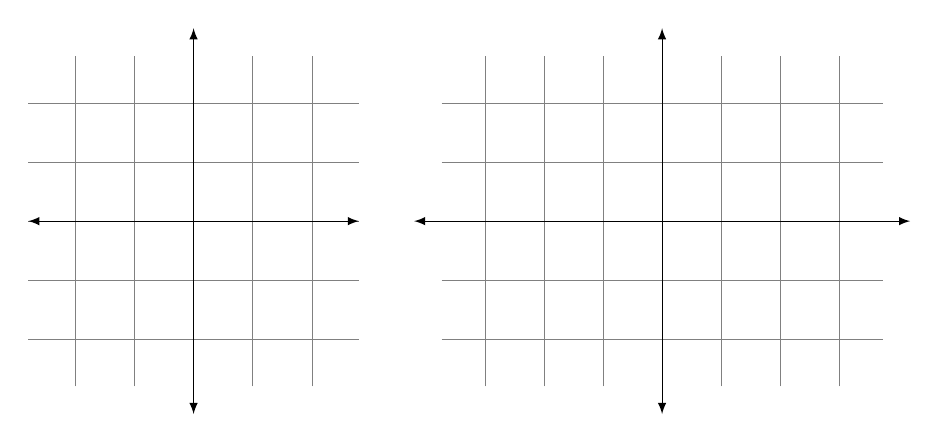
\begin{tikzpicture}[x={(.7cm,0)},y={(0,.7cm)},>=latex]

	\begin{scope}
		\draw [ultra thin,gray,step=.75cm] (-3,-3) grid (3,3);
		\draw [<->] (-3,0) -- (3,0);
		\draw [<->] (0,-3.5) -- (0,3.5);
		\vmispider[very thick];
	\end{scope}

	\begin{scope}[shift={(8.5,0)}]
		\draw [ultra thin,gray,step=.75cm] (-4,-3) grid (4,3);
		\draw [<->] (-4.5,0) -- (4.5,0);
		\draw [<->] (0,-3.5) -- (0,3.5);
		\vmispider[very thick,cm={0,-.5,1.5,0,(0,0)}]
	\end{scope}

\end{tikzpicture}
\end{center}
\mycaption{Transforming the Cartesian plane in Example \ref{ex_transf_2}}
\label{fig:transf_2_2}
\end{myfigure}
\vskip -2\baselineskip}

\medskip

Right now we are focusing on transforming the Cartesian plane -- we are making 2D transformations. Knowing how to do this provides a foundation for transforming 3D space, which, among other things, is very important when producing 3D computer graphics. Basic shapes can be drawn and then rotated, stretched, and/or moved to other regions of space. This also allows for things like ``moving the camera view.'' Of course, algebraically, there is nothing stopping us from working with transformations of vectors in $\mathbb{R}^n$ for \textit{any} value of $n$. The limitation to two and three dimensions is strictly one of visualization.

What kinds of transformations are possible? We have already seen some of the things that are possible: rotations, stretches, and flips. We have also mentioned some things that are not possible. For instance, we stated that straight lines always get transformed to straight lines. Therefore, we cannot transform the unit square into a circle using a matrix.

Let's look at some common transformations of the Cartesian plane and the matrices that perform these operations. In the following figures, a transformation matrix will be given alongside a picture of the transformed unit square. (The original unit square is drawn lightly as well to serve as a reference.)\\

%\pagebreak

\noindent \large \textsf{\textbf{ 2D Matrix Transformations}} \normalsize\\ \label{page:plane_transformations}

\begin{minipage}{.3\linewidth}
\raggedright\textbf{Horizontal stretch} by a factor of $k$.
\[
\bmx{cc}k&0\\0&1\emx
\]
\end{minipage}
\begin{minipage}{.7\linewidth}
\begin{center}

\begin{tikzpicture}[>=latex]
		\drawxlines{-1}{2.5}{1,2};
		\drawylines{-1}{2.5}{1,2};
		\begin{scope}[opacity=.5]\unitsquare[very thin];\end{scope}
		\unitsquare[thick,cm={1.5,0,0,1,(0,0)}];
		\node [above] at (C) {$(k,1)$};
\end{tikzpicture}
\end{center}
\end{minipage}

\vskip .5cm
\hrule
\vskip .5cm

\begin{minipage}{.3\linewidth}
\raggedright\textbf{Vertical stretch} by a factor of $k$.
\[
\bmx{cc}1&0\\0&k\emx
\]
\end{minipage}
\begin{minipage}{.7\linewidth}
\begin{center}

\begin{tikzpicture}[>=latex]
		\drawxlines{-1}{2.5}{1,2};
		\drawylines{-1}{2.5}{1,2};
		\begin{scope}[opacity=.5]\unitsquare[very thin];\end{scope}
		\unitsquare[thick,cm={1,0,0,1.5,(0,0)}];
		\node [above] at (C) {$(1,k)$};
\end{tikzpicture}
\end{center}
\end{minipage}


\vskip .5cm
\hrule
\vskip .5cm

\begin{minipage}{.3\linewidth}
\raggedright\textbf{Horizontal shear} by a factor of $k$.
\[
\bmx{cc}1&k\\0&1\emx
\]
\end{minipage}
\begin{minipage}{.7\linewidth}
\begin{center}

\begin{tikzpicture}[>=latex]
		\drawxlines{-1}{2.5}{1,2};
		\drawylines{-1}{2.5}{1,2};
		\begin{scope}[opacity=.5]\unitsquare[very thin];\end{scope}
		\unitsquare[thick,cm={1,0,1.5,1,(0,0)}];
		\node [above] at (D) {$(k,1)$};
\end{tikzpicture}
\end{center}
\end{minipage}

\vskip .5cm
\hrule
\vskip .5cm

\begin{minipage}{.3\linewidth}
\raggedright\textbf{Vertical shear} by a factor of $k$.
\[
\bmx{cc}1&0\\k&1\emx
\]
\end{minipage}
\begin{minipage}{.7\linewidth}
\begin{center}

\begin{tikzpicture}[>=latex]
		\drawxlines{-1}{2.5}{1,2};
		\drawylines{-1}{2.5}{1,2};
		\begin{scope}[opacity=.5]\unitsquare[very thin];\end{scope}
		\unitsquare[thick,cm={1,1.5,0,1,(0,0)}];
		\node [right] at (B) {$(k,1)$};
\end{tikzpicture}
\end{center}
\end{minipage}

\vskip .5cm
\hrule
\vskip .5cm

\begin{minipage}{.3\linewidth}
\raggedright\textbf{Horizontal reflection} across the $y$ axis.
\[
\bmx{cc}-1&0\\0&1\emx
\]
\end{minipage}
\begin{minipage}{.7\linewidth}
\begin{center}

\begin{tikzpicture}[>=latex]
		\drawxlines{-1.5}{1.5}{1,-1};
		\drawylines{-1.5}{1.5}{1,-1};		
		\begin{scope}[opacity=.5]\unitsquare[very thin];\end{scope}
		\unitsquare[thick,cm={-1,0,0,1,(0,0)}];
\end{tikzpicture}
\end{center}
\end{minipage}

\vskip .5cm
\hrule
\vskip .5cm

\begin{minipage}{.3\linewidth}
\raggedright\textbf{Vertical reflection} across the $x$ axis.
\[
\bmx{cc}1&0\\0&-1\emx
\]
\end{minipage}
\begin{minipage}{.7\linewidth}
\begin{center}

\begin{tikzpicture}[>=latex]
\drawxlines{-1.5}{1.5}{1,-1};
		\drawylines{-1.5}{1.5}{1,-1};	
		\begin{scope}[opacity=.5]\unitsquare[very thin];\end{scope}
		\unitsquare[thick,cm={1,0,0,-1,(0,0)}];
\end{tikzpicture}
\end{center}
\end{minipage}

\vskip .5cm
\hrule
\vskip .5cm

\begin{minipage}{.3\linewidth}
\raggedright\textbf{Diagonal reflection} across the line $y=x$.
\[
\bmx{cc}0&1\\1&0\emx
\]
\end{minipage}
\begin{minipage}{.7\linewidth}
\begin{center}

\begin{tikzpicture}[>=latex]
		\drawxlines{-1.5}{1.5}{1,-1};
		\drawylines{-1.5}{1.5}{1,-1};	
		\begin{scope}[opacity=.5]\unitsquare[very thin];\end{scope}
		\draw [very thin,gray,dashed] (-1,-1) -- (1.5,1.5);
		\unitsquare[thick,cm={0,1,1,0,(0,0)}];
\end{tikzpicture}
\end{center}
\end{minipage}

\vskip .5cm
\hrule
\vskip .5cm

\begin{minipage}{.3\linewidth}
\raggedright\textbf{Rotation} around the origin by an angle of $\theta$.
\[
\bmx{cc}\cos \theta & -\sin \theta \\ \sin \theta & \cos \theta  \emx
\]
\end{minipage}
\begin{minipage}{.7\linewidth}
\begin{center}

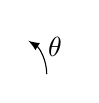
\begin{tikzpicture}[>=latex]
		\drawxlines{-1.5}{1.5}{1,-1};
		\drawylines{-.5}{2.5}{1,2};	
		\begin{scope}[opacity=.5]\unitsquare[very thin];\end{scope}
		\unitsquare[thick,cm={0.5,0.866,-0.866,0.5,(0,0)}];
		\draw [->] (.5,0) arc (0:58:0.5cm) ;
		\path (.7,0) arc (0:30:.7) node {$\theta$};
\end{tikzpicture}
\end{center}
\end{minipage}

\vskip .5cm
\hrule
\vskip .5cm

\begin{minipage}{.3\linewidth}
\raggedright\textbf{Projection} onto the $x$ axis.

(Note how the square is ``squashed'' down onto the $x$-axis.)

\[
\bmx{cc}1&0\\0&0  \emx
\]
\end{minipage}
\begin{minipage}{.7\linewidth}
\begin{center}

\begin{tikzpicture}[>=latex]
		\drawxlines{-1.5}{1.5}{1,-1};
		\drawylines{-1.5}{1.5}{1,-1};	
		\begin{scope}[opacity=.5]\unitsquare[very thin];\end{scope}
		\unitsquarewithoutarrows[thick,cm={1,0,0,0,(0,0)}];
		%\filldraw (A)[shift={(-2pt,0)}] arc (-180:0:2pt);
		%\filldraw [red] (B)[shift={(-2pt,0)}] arc (-180:0:2pt);
\end{tikzpicture}
\end{center}
\end{minipage}

\vskip .5cm
\hrule
\vskip .5cm

\begin{minipage}{.3\linewidth}
\raggedright\textbf{Projection} onto the $y$ axis.

(Note how the square is ``squashed'' over onto the $y$-axis.)

\[
\bmx{cc}0&0\\0&1  \emx
\]
\end{minipage}
\begin{minipage}{.7\linewidth}
\begin{center}

\begin{tikzpicture}[>=latex]
		\drawxlines{-1.5}{1.5}{1,-1};
		\drawylines{-1.5}{1.5}{1,-1};	
		\begin{scope}[opacity=.5]\unitsquare[very thin];\end{scope}
		\unitsquarewithoutarrows[thick,cm={0,0,0,1,(0,0)}];
		%\filldraw[shift={(-2pt,-2pt)}] (A)[shift={(0,2pt)}] arc (90:270:2pt);
		%\filldraw [blue] (C)[shift={(0,-2pt)}] arc (-90:90:2pt);
\end{tikzpicture}
\end{center}
\end{minipage}

\vskip 1cm

Now that we have seen a healthy list of transformations that we can perform on the Cartesian plane, let's practice a few more times creating the matrix that gives the desired transformation. In the following example, we develop our understanding one more critical step.

\pagebreak

\example{ex_transf_3}{Determining the matrix of a transformation}{Find the matrix \tta\ that transforms the Cartesian plane by performing the following operations in order:

\begin{minipage}[t]{.4\linewidth}
\begin{enumerate}
	\item Vertical shear by a factor of 0.5
	\item	Counterclockwise rotation about the origin by an angle of $\theta = 30^\circ$
\end{enumerate}
\end{minipage}
\begin{minipage}[t]{.4\linewidth}
\begin{enumerate}\addtocounter{enumi}{2}
	\item	Horizontal stretch by a factor of 2
	\item	Diagonal reflection across the line $y=x$
	\end{enumerate}
\end{minipage}
}
{Wow! We already know how to do this -- sort of. We know we can find the columns of \tta\ by tracing where \veone\ and \vetwo\ end up, but this also seems difficult. There is so much that is going on. Fortunately, we can accomplish what we need without much difficulty by being systematic.

First, let's perform the vertical shear. The matrix that performs this is 
\[
\tta_1 = \bmx{cc}1&0\\0.5&1\emx.
\]
After that, we want to rotate everything clockwise by $30^\circ$. To do this, we use 
\[
\tta_2 = \bmx{cc} \cos 30^\circ & -\sin 30^\circ\\ \sin 30^\circ & \cos 30^\circ \emx = \bmx{cc} \sqrt{3}/2 & -1/2 \\ 1/2 & \sqrt{3}/2\emx.
\]
In order to do both of these operations, in order, we multiply $\tta_2\tta_1$. 

\mnote{.5}{\textbf{Note:} recall from Section \ref{sec:matrix_multiplication} that matrix multiplication is \textbf{not} commutative. Since $A_1A_2\neq A_2A_1$ in general, we should expect that the transformation $A_2(A_1\vec x) = (A_2A_1)\vec x$ is not the same as the transformation $A_1(A_2\vec x) = (A_1A_2)\vec x$. Interpreted as transformations of the plane, this makes sense visually: for example, in most cases, a reflection followed by a rotation will not produce the same result as performing the rotation first, followed by the reflection. The reader is encouraged to experiment with a few examples to see what happens when the order is reversed. } 

%\drawexampleline{ex_transf_3}

To perform the final two operations, we note that 
\[
\tta_3 = \bmx{cc}2&0\\0&1\emx \quad \text{ and } \quad \tta_4 = \bmx{cc} 0&1 \\ 1&0\emx
\]
perform the horizontal stretch and diagonal reflection, respectively. Thus to perform all of the operations ``at once,'' we need to multiply by 
\begin{align*} \tta &= \tta_4\tta_3\tta_2\tta_1 \\
										& = \bmx{cc} 0&1 \\ 1&0\emx\bmx{cc}2&0\\0&1\emx\bmx{cc} \sqrt{3}/2 & -1/2 \\ 1/2 & \sqrt{3}/2\emx\bmx{cc}1&0\\0.5&1\emx \\
										& = \bmx{cc} (\sqrt{3}+2)/4 & \sqrt{3}/2 \\ (2\sqrt{3}-1)/2 & -1\emx\\
										& \approx \bmx{cc} 0.933 & 0.866\\ 1.232 & -1 \emx.
\end{align*}

Let's consider this closely. Suppose I want to know where a vector \vx\ ends up. We claim we can find the answer by multiplying $\tta\vx$. Why does this work? Consider:
%\drawexampleline
\enlargethispage{2\baselineskip}
\begin{align*}
\tta\vx &= \tta_4\tta_3\tta_2\tta_1\vx \\
				&= \tta_4\tta_3\tta_2(\tta_1\vx) & &\textsf{\hskip 20pt  \small(performs the vertical shear)}\hfill \\
				&= \tta_4\tta_3(\tta_2\vx_1) & &\textsf{\hskip 20pt  \small(performs the rotation)}\hfill\\
				&= \tta_4(\tta_3\vx_2) & &\textsf{\hskip 20pt  \small(performs the horizontal stretch)}\hfill\\
				&= \tta_4\vx_3 & &\textsf{\hskip 20pt  \small(performs the diagonal reflection)}\hfill\\
				&= \vx_4 & &\textsf{\hskip 20pt  \small(the result of transforming $\vx$)}\hfill \\
\end{align*}

Most readers are not able to visualize exactly what the given list of operations does to the Cartesian plane. In Figure \ref{fig:trans_3_1} we sketch the transformed unit square; in Figure \ref{fig:trans_3_2} we sketch a shape and its transformation.

\begin{myfigure}
\begin{center}
\begin{tikzpicture}[>=latex]
		\drawxlines{-.5}{2.5}{1,2};
		\drawylines{-1.5}{1.5}{-1,1};
		\begin{scope}[opacity=.5]\unitsquare[very thin];\end{scope}
		\unitsquare[thick,cm={0.933,1.232,0.866,-1,(0,0)}];
\end{tikzpicture}
\end{center}
\mycaption{The transformed unit square in Example \ref{ex_transf_3}.}
\label{fig:trans_3_1}
\end{myfigure}

\begin{myfigure}
\begin{center}
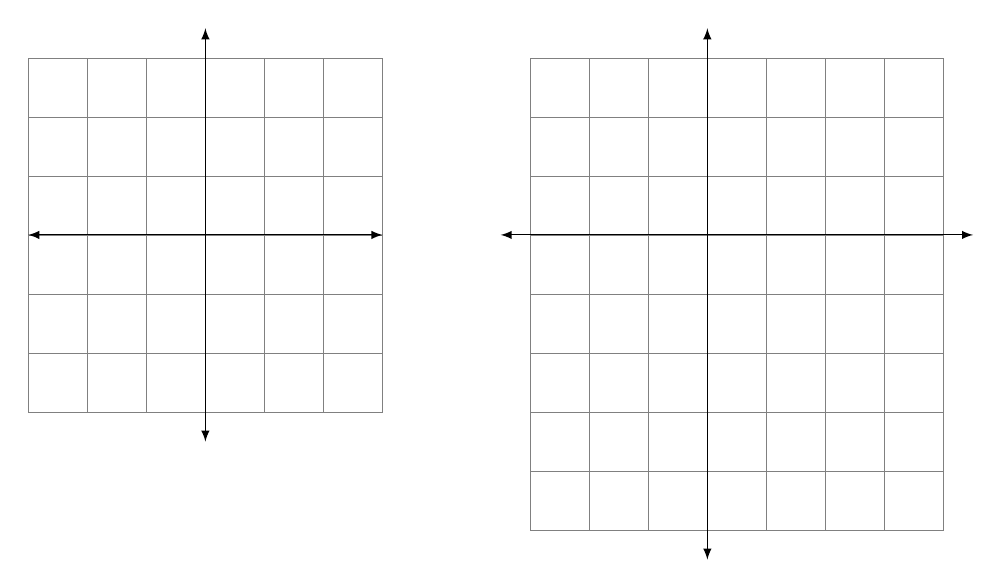
\begin{tikzpicture}[x={(.75cm,0)},y={(0,.75cm)},>=latex]
		\begin{scope}
	\draw [ultra thin,gray,step=.75cm] (-3,-3) grid (3,3);
	\draw [<->] (-3,0) -- (3,0);
	\draw [<->] (0,-3.5) -- (0,3.5);
	\vmispider[very thick];
\end{scope}
\begin{scope}[shift={(8.5,0)}]
	\draw [ultra thin,gray,step=.75cm] (-3,-5) grid (4,3);
	\draw [<->] (-3.5,0) -- (4.5,0);
	\draw [<->] (0,-5.5) -- (0,3.5);
	\vmispider[very thick,cm={0.933,1.232,0.866,-1,(0,0)}];
\end{scope}
\end{tikzpicture}
\end{center}
\mycaption{A transformed shape in Example \ref{ex_transf_3}.}
\label{fig:trans_3_2}
\end{myfigure}
\vskip -2\baselineskip}

\medskip

Once we know what matrices perform the basic transformations, (or know where to find them) performing complex transformations on the Cartesian plane really isn't that $\ldots$ complex. It boils down to multiplying by a series of matrices. 

We've shown many examples of transformations that we can do, and we've mentioned just a few that we can't -- for instance, we can't turn a square into a circle. Why not? Why is it that straight lines get sent to straight lines? 
All these questions require us to think like mathematicians -- we are being asked to study the \textit{properties} of an object we just learned about and their connections to things we've already learned. We'll do all this (and more!) in the following section.\\

%\clearpage


\printexercises{exercises/05_03_exercises}

